\chapter{Cause-Effect Graphs: Syntax and Semantics}
\label{ch:syntax-and-semantics}

\section{Defining Cause-Effect Graphs}

Let's take a closer look at Cause-Effect graphs. These graphs are visual tools used to model the logical relationships between a system's inputs and outputs, where the inputs represent the causes and the outputs represent the effects. They are especially useful for capturing and visualizing the decision-making logic in complex systems, making them highly valuable for business-critical applications \cite{ceg}.

\begin{itemize}
	\item \textbf{Causes} represent conditions or inputs to the system, which can be external stimuli or internal states that trigger certain actions.
	\item \textbf{Effects} represent the resulting actions, decisions, or outputs that occur as a consequence of the specified causes.
\end{itemize}

A cause-effect graph maps the interdependencies between these inputs and outputs, where each connection between a cause and an effect represents a logical relationship, often described in terms of \textbf{Boolean} logic. These logical relationships are typically expressed using basic logical operators such as AND, OR, and NOT, which define how different causes combine to produce specific effects.

\subsection{Key Components of a Cause-Effect Graph}

\begin{enumerate}
	\item \textbf{Nodes}
	      \begin{itemize}
		      \item The nodes represent the causes and the effects of the graph.
		      \item Each node in the graph can be represented as a Boolean expression and can either be true or false, reflecting the presence or absence of a condition or outcome.
	      \end{itemize}
	\item \textbf{Edges}
	      \begin{itemize}
		      \item Directed edges connect causes to effects, illustrating the logical dependency between them. The edges represent the conditions under which an effect occurs, based on the combination of the cause inputs.
	      \end{itemize}
	\item \textbf{Logical Operators}
	      \begin{itemize}
		      \item The relationships between causes and effects are typically governed by logical operators. Mostly three of them are used:
		            \begin{itemize}
			            \item \textbf{AND}: The effect occurs only if all connected causes are true.
			            \item \textbf{OR}: The effect occurs if at least one of the connected causes is true.
			            \item \textbf{NOT}: An effect occurs if the connected cause is false. These operators allow testers and developers to model complex dependencies in a concise and structured way.
		            \end{itemize}
	      \end{itemize}
	\item \textbf{Constraints}
		  \begin{itemize}
		      \item Constraints may be applied to causes and effects, such as mutually exclusive conditions or specific combinations of causes that must or must not occur together.
		  \end{itemize}
\end{enumerate}

\subsection{Syntax and Semantics of Cause-Effect Graphs}

The graph outlines the causes, effects, and the relationships between them. Each node represents a valid system input or output, and each edge corresponds to a logical operation that adheres to \textbf{Boolean} algebra. These graph constraints define the syntax of a cause-effect graph.

The syntax of the representation is relatively simple, but the underlying meaning and corresponding business logic can be complex. The semantics of the graph describe how the relationships between the causes and effects are interpreted during testing or system evaluation. When evaluating a cause-effect graph, the truth values of the input causes are propagated through the graph according to the logical operators, resulting in the determination of the truth values for the output effects.

In practice, cause-effect graphs serve as a high-level representation of business rules, helping to capture all potential interactions between inputs and outputs. These graphs can be converted into formal logic expressions, which are then used to generate test cases. The objective is to model the business logic using this graphing technique and ensure test coverage by addressing all possible combinations of causes and effects.

\begin{figure}[H]
	\centering
	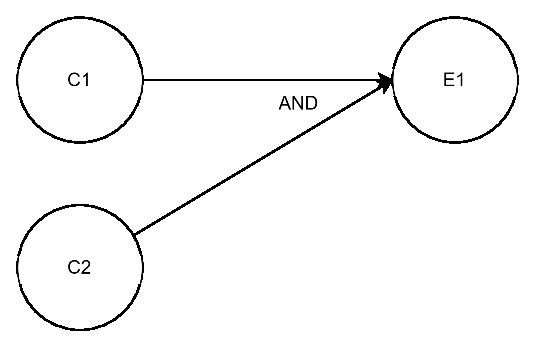
\includegraphics[width=0.4\textwidth,height=100px]{BasicCauseEffect}
	\caption{A basic Cause-Effect graph with AND logical relation}
	\label{fig:basic-cause-effect}
\end{figure}


\section{Proposed Syntax}

The proposed syntax for cause-effect graphs is designed to be both intuitive and flexible, allowing for the clear representation of complex business logic while maintaining a structured approach to logical relationships. The syntax focuses on defining nodes, edges, and logical operators that model the interaction between causes and effects. The aim is to develop a system that can be readily converted into formal logic expressions and simplifies the process of describing the graph in a scripted format.

\subsection{Key Components of the Proposed Syntax}

\subsubsection{Nodes}

\begin{itemize}
	\item \textbf{Cause Nodes (C)}: Represent the input conditions, triggers, or events that lead to certain effects. These can be any factors that influence the system's behavior, such as user inputs, external events, or internal states.
	\item \textbf{Effect Nodes (E)}: Represent the outcomes, results, or actions triggered by specific causes. These effects are the observable consequences within the system that occur based on the logical relationships defined.
	\item \textbf{Logical Nodes}: Represent a logical relationship between two or more cause nodes, logical nodes, or a transformations of cause or logical nodes.
\end{itemize}

Each node is labeled as either a cause (C) or an effect (E), with unique identifiers such as C1, C2, ..., or E1, E2, ..., to distinguish between multiple causes and effects. Logical nodes are also labeled with the corresponding logical operation: NOT, AND, or OR.

\subsubsection{Edges}

\begin{itemize}
	\item \textbf{Directed Edges}: An arrow represents a connection between two nodes, indicating a one-way relationship from the source node to the destination node. These nodes illustrate the logical dependencies between them. A cause node can only act as a source node, not a destination, and an effect node can only serve as a destination node, not a source.
	\item \textbf{Logical Edges}: In this proposal, there are no logical edges. Instead, the edge types are transformed into logical nodes.
\end{itemize}

\subsubsection{Logical Operators}

\begin{itemize}
	\item \textbf{AND}: The effect occurs only if all connected causes are true. For example, if $ C1 \land C2 \rightarrow E1 $, the effect E1 will only happen when both C1 and C2 are true.
	\item \textbf{OR}:The effect occurs if at least one of the connected causes is true. For instance, $ C1 \lor C2 \rightarrow E1 $ indicates that E1 will occur if either C1 or C2 is true.
	\item \textbf{NOT}: The effect occurs if the connected cause is false. For example, $ \lnot C1 \rightarrow E1 $ means that E1 will happen if C1 is false.
\end{itemize}

\subsubsection{Grouping and Hierarchy}

\begin{itemize}
	\item \textbf{Nested Conditions}: The syntax allows for nested conditions to represent more complex logic, where certain effects depend on combinations of causes that are themselves the result of other causes. For example, $ ((C1 \land C2) \lor C3) \rightarrow E1 $ models a more complex interaction.
	\item \textbf{Grouping}: Causes or effects can be grouped together when they share common logical conditions, simplifying the visual representation and improving clarity.
\end{itemize}

\subsection{Example}

In this proposed syntax, a simple cause-effect relationship could be represented as follows:

\begin{compactitem}
	\item C1 AND C2 cause E1: $ (C1 \land C2) = E1 $
	\item C1 OR C3 cause E2: $ (C1 \lor C3) = E2 $
	\item NOT C4 causes E3: $ \lnot C4 = E3 $
	\item NOT C1 OR C2 cause E4: $ (\lnot C1 \lor C2) = E4 $
\end{compactitem}

These relationships define how the system should behave under different combinations of input conditions, and the structure allows for easy transformation into formal logic.

\subsection{Benefits of the Proposed Syntax}

\begin{itemize}
	\item \textbf{Clarity}: Clearly distinguishes between causes, logical operations and effects, making the logical rules easier to interpret.
	\item \textbf{Scalability}: Supports complex logic with nested conditions, allowing it to scale to larger systems.
	\item \textbf{Test Case Generation}: By translating the graph into formal logic expressions, the syntax enables automated generation of test cases.
	\item \textbf{Flexibility}: Provides enough flexibility to model a wide range of logical systems, from simple rules to highly complex interactions.
\end{itemize}

The proposed syntax aims to strike a balance between simplicity and expressiveness.

\section{Proposed Semantics}

The semantics of cause-effect graphs define how the logical relationships between causes and effects are interpreted and evaluated. These semantics guide the process of converting the graph into formal logic expressions that can be used for automated test generation. The primary goal of the proposed semantics is to ensure a clear, consistent, and systematic interpretation of the cause-effect relationships in a way that models the underlying business logic accurately.

\subsection{Key Aspects of the Proposed Semantics}

\begin{enumerate}
	\item \textbf{Evaluation of Causes}
		
		Each cause node represents a condition or input that can either be true or false. The system evaluates the truth value of each cause based on the current state of inputs. These evaluations are binary, where:
		\begin{itemize}
			\item \textbf{True (1)}: The condition is met, or the input is active.
			\item \textbf{False (0)}: The condition is not met, or the input is inactive.
		\end{itemize}
	\item \textbf{Effect Determination}
		\begin{itemize}
			\item Each effect node represents an outcome that occurs if the corresponding causes satisfy the logical relationships defined by the graph. The evaluation of an effect depends on the truth values of the connected causes and the logical operators that link them.
			\item If the conditions for an effect are met (the causes and logical relationships evaluate to true), the effect is triggered or considered true. If not, the effect remains false.
		\end{itemize}
	\item \textbf{Propagation of Truth Values}
		
		The truth values of the cause nodes propagate through the graph according to the logical operators (AND, OR, NOT) used to connect them to the effect nodes:
		\begin{itemize}
			\item \textbf{AND}: The effect is true only if all connected causes are true. For example, if the causes C1 and C2 are both true, then the effect E1 ($ C1 \land C2 = E1 $) will also be true.
			\item \textbf{OR}: The effect is true if at least one of the connected causes is true. For instance, if either C1 or C3 is true, the effect E2 ($ C1 \lor C3 = E2 $) will be true.
			\item \textbf{NOT}: The effect is true if the connected cause is false. For example, if C4 is false, then the effect E3 ($ \lnot C4 = E3 $) will be true.
		\end{itemize}
	\item \textbf{Handling Complex Conditions}
		\begin{itemize}
			\item For graphs with nested conditions or multiple layers of logical relationships, the truth values of intermediate nodes (representing partial conditions) are calculated first and then propagated to the next level of the graph. This hierarchical evaluation ensures that the overall business logic is respected.
			\item For example, if the graph contains a complex condition such as $ ((C1 \land C2) \lor C3) = E1 $, the truth value of $ (C1 \land C2) $ is first evaluated before combining it with C3 to determine whether E1 is true.
		\end{itemize}
	\item \textbf{Boolean Logic Interpretation}
		
		The proposed semantics align with Boolean logic, ensuring that each cause-effect relationship can be translated into a formal logic expression. These expressions take the form of Boolean equations that model the decision-making process of the system. For example:
		\begin{itemize}
			\item $ (C1 \land C2) = E1 $ translates to a Boolean expression where C1 and C2 equal with E1.
			\item $ \lnot C4 = E3 $ means that C4 not equals with E3.
		\end{itemize}	
\end{enumerate}

\subsection{Benefits of the Proposed Semantics}

\begin{itemize}
	\item \textbf{Accuracy}: Ensures that all cause-effect relationships are evaluated logically and consistently, reducing the risk of incorrect test case generation.
	\item \textbf{Automation-Friendly}: The clear Boolean logic interpretation allows for seamless translation into automated test generation frameworks.
	\item \textbf{Scalability}: Supports complex and nested conditions, making it suitable for large-scale business systems with intricate dependencies.
	\item \textbf{Flexibility}: Adapts to systems with time or state dependencies, as well as handling indeterminate values.
\end{itemize}

In summary, the proposed semantics ensure a rigorous and consistent evaluation of cause-effect relationships, enabling effective modeling of business logic and facilitating comprehensive, automated testing.

\section{Examples}

To illustrate the practical application of cause-effect graphs, let's consider a few examples that demonstrate how business logic can be modeled and translated into testable logical expressions.

\subsection{Example 1}

\begin{table}[H]
	\centering
	\begin{tabular}{ | m{0.1\textwidth} | m{0.1\textwidth} | m{0.65\textwidth} | }
		\hline
		\textbf{Name} & \textbf{Type} & \textbf{Description} \\
		\hline \hline
		C1 & Cause & User enters valid login credentials. \\
		\hline
		C2 & Cause & User has a valid account. \\
		\hline
		E1 & Effect & User is granted access. \\
		\hline
	\end{tabular}
	\caption{Graph Example 1 - Table of nodes}
	\label{tab:graph-example-1}
\end{table}

Both cause, C1 and C2, must be true for the effect, E1, to occur. The logical relationship can be expressed as: $ C1 \land C2 = E1 $.

\begin{figure}[H]
	\centering
	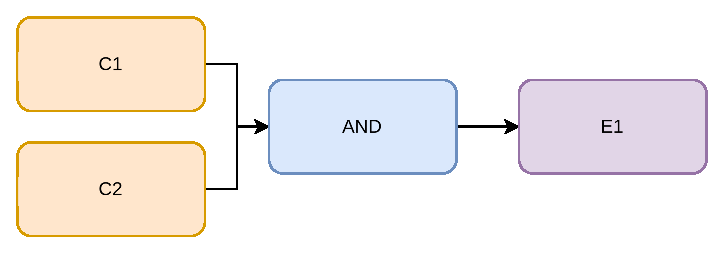
\includegraphics[width=0.6\textwidth,height=100px]{Example_1}
	\caption{Graph Example 1 - Visualized graph}
	\label{fig:graph-example-1}
\end{figure}

\subsection{Example 2}

\begin{table}[H]
	\centering
	\begin{tabular}{ | m{0.1\textwidth} | m{0.1\textwidth} | m{0.65\textwidth} | }
		\hline
		\textbf{Name} & \textbf{Type} & \textbf{Description} \\
		\hline \hline
		C1 & Cause & User enters a valid username. \\
		\hline
		C2 & Cause & User enters a valid password. \\
		\hline
		C3 & Cause & User enters a valid two-factor authentication code. \\
		\hline
		E1 & Effect & User is granted access. \\
		\hline
		E2 & Effect & System sends a warning if only username and password are correct without the two-factor authentication. \\
		\hline
	\end{tabular}
	\caption{Graph Example 2 - Table of nodes}
	\label{tab:graph-example-2}
\end{table}

Here, E1 only occurs if C1, C2, and C3 are all true. However, E2 occurs if C1 and C2 are true, but C3 is false. 

\begin{compactitem}
	\item $ (C1 \land C2 \land C3) = E1 $
	\item $ (C1 \land C2 \land \lnot C3) = E1 $
\end{compactitem}

\begin{figure}[H]
	\centering
	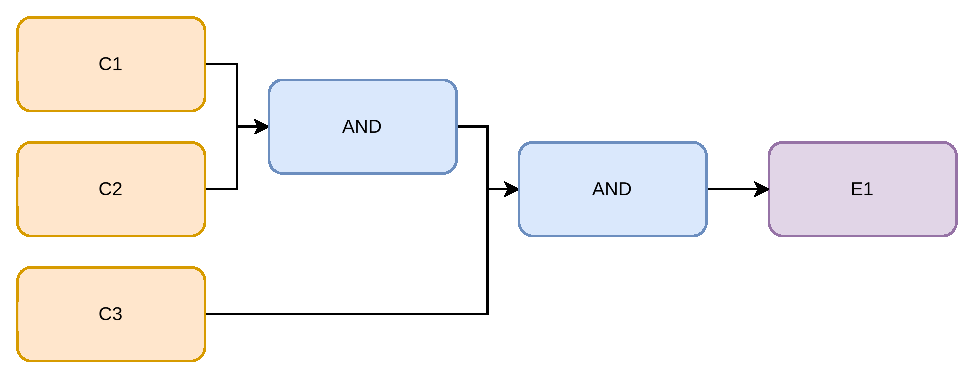
\includegraphics[width=0.7\textwidth,height=140px]{Example_2_1}
	\caption{Graph Example 2 - Visualized graph for Rule 1}
	\label{fig:graph-example-2-1}
\end{figure}

\begin{figure}[H]
	\centering
	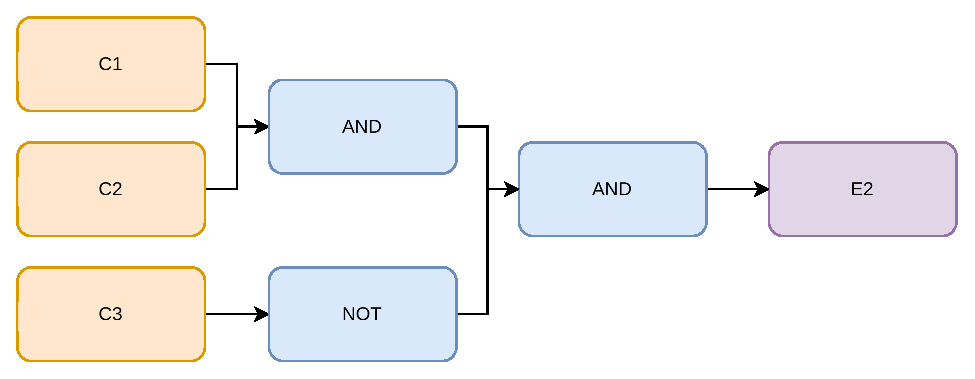
\includegraphics[width=0.7\textwidth,height=140px]{Example_2_2}
	\caption{Graph Example 2 - Visualized graph for Rule 2}
	\label{fig:graph-example-2-2}
\end{figure}

\subsection{Summary of Examples}

These examples demonstrate how cause-effect graphs can be constructed and used to model business logic in software systems. By using logical operators (AND, OR, NOT), the graphs can capture a wide range of conditions and dependencies, which can then be transformed into formal logic expressions for test generation. Each example highlights how different types of business logic (simple, complex, nested) can be represented visually.